\documentclass{article}
\usepackage[utf8]{inputenc}
\usepackage{hyperref}
\usepackage[utf8]{inputenc}
\usepackage{graphicx}

\title{Parallel Exam 1}
\author{Jennifer Kulich }
\date{October 19, 2020}

\begin{document}

\maketitle
\section{A Little Background}
I'm not really sure how to approach this, but I was only able to finish so much of the exam. I had been super busy with tests and Senior Design that I wasn't able to start until mid last week. I was able to get the algorithm and OpenMP working, and I knew I'd be able to get the CUDA part done Friday, Saturday, and Sunday given I had enough time. I started working on it, and early Saturday morning, my roommates reset the wifi in our apartment, and I couldn't connect anymore. I spent most of my Saturday morning at the vet (my cat got very sick this past week) and waiting for my password only to find out that they had created a whitelist, and the roommate who had the router in her room refused to do anything about it. I gave her instructions on how to reset things in case she did this by accident, but she ignored me. By that point, most of my Saturday had gone by, and I hadn't been able to work on the CUDA part of things. I've been having a lot of troubles with this roommate, and it's gotten to the point where I'm mentally exhausted. I was looking at moving out, but everything in Rapid is so expensive, and this past week my cat was at the vet what felt like almost every day. I think her turning off the wifi was retaliation for me not moving out, but I'm just so burnt out, and now I'm scrambling to find a new place to live because I'm so miserable. I tried my best to write something for the CUDA part of the program (I was able to find a place with wifi on Sunday), but I don't even know if it compiles. I know the Floyd's algorithm works. 
I'm really sorry. I'm not trying to create excuses for why it's not done, and I really don't want more time to work on it because I'm so stressed right now and I'm trying to move. I just thought I'd let you know so you wouldn't spend too much time looking at my code.

\section{The Program}
The program was to use Floyd's algorithm to find the shortest path. One program will utilize OpenMP, and the other will utilize CUDA. 

\section{What was Submitted and How to Run}
\subsection{OpenMP}
In the OpenMP file, there's the Floyds.c file and Makefile. To run this, do "make clean" and then "make all". After that,  you can type ./floyds {number vertices} where you input the number of vertices in the graph. The program will print out the randomly generated graph and the result from Floyd's algorithm. It will also print out timing information which is used for data analysis and for your own knowledge. If you would like to change the thread count, you can simply go into the .c file and change the variable THREAD\_COUNT.
\subsection{CUDA}
Again, I haven't even tried to compile it, so I don't know how that would work.

\section{Algorithms and Libraries Used}
The code for Floyd's algorithm was taken from \href{https://www.geeksforgeeks.org/floyd-warshall-algorithm-dp-16/ }{Geeks for Geeks} The algorithm itself was easy to understand. 
For the OpenMp project, I started a timer that would time everything. This would be used for the data analysis at the end. I then got the number of vertices for the graph from the user and created the graph. To get the P(there is an edge) = 0.25, I took a random number, modded it by 4, and if the number was a multiple of 4, it would get assigned a random number between 1 and 20 which represented the distance. Anything else got INF. I also printed off this graph so you could see the start. I then passed this into the Floyd's algorithm, started the timer for the parallel part, did the algorithm, stopped the parallel time, printed the graph, stopped the other timer, and calculated the efficiency and speedup for data analysis. To do all of this, I used stdio.h, time.h, omp.h, stdlib.h, math.h, and limits.h libraries. 


\section {Functions and Program Structure}
\subsection{OpenMP}
In main, the random graph is made based on the number of vertices passed in. This will also print the graph so the user can see what the initial graph looked like. Then, the Floyd's algorithm is called. In the algorithm function, the final graph will be printed by calling a function, and the time it took to run the parallel section will be printed. Back in main, the program will print the total time it took to run everything and then call another function to print out the efficiency and speedup of the program.
\subsection{CUDA}
The layout is the same as the OpenMP program minus a small difference. Instead of doing all 3 for loops in one function, I put the inner two loops into a separate function. Before I went into that separate function, I would need to copy the graph to the GPU, and after getting back from that separate function, I would need to copy the graph back to the host.

\section{Testing and Verification Process}
For testings, I first wrote out the algorithm, didn't make it parallel, and hardcoded the example graphs. Once I determined that the algorithm was correct, I made the program parallel and tested again with the hardcoded graphs. Once I was sure that I was getting the right answers, I took out the hardcoded graphs and made randomly generated graphs. This worked very well for me and helped me feel confident with my code. (see figure 1)


\section{Data}
We were supposed to do data analysis of speed-up and efficiency. Speedup was defined as the ((serial portion + parallel portion)) / serial portion + (parallel portion / number of processors)) . The efficiency was defined as the ((serial portion + parallel portion)) / ((serial portion * number of processors) + parallel portion)). To find the serial portion, I took the time to execute the whole program - time to execute the parallel portion. This made gathering data easy.

\section{Analysis of Data}
So this was the part where I realized that I don't know what I'm doing when it comes to using Excel... I tried making graphs, but things turned out weird. If I get the time, I'll make graphs and hopefully take out this commentary. 
\subsection{OpenMP}
I ran the program on powers of 2 threads starting with 8 threads going all the way up to 512 threads. For each one of those, I ran graphs with vertices increasing by 10's going from 10 vertices to 70 vertices. See figure 2 for data. In terms of efficiency, it was pretty clear that as the number of threads increased, the efficiency went down. It didn't seem to matter how many vertices there were after a while- in fact, the efficiency almost became all the same. Regardless of the speedup, it's clear that a lower amount of threads would be the best to solve a graph with a variable amount of vertices.

\begin{figure}
    \centering
    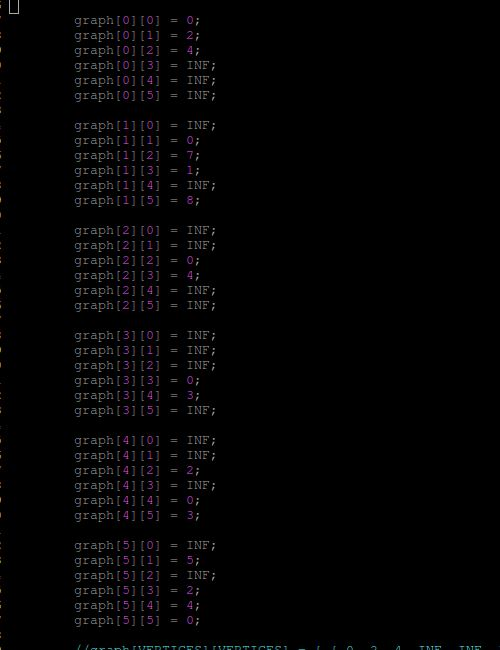
\includegraphics[width=4cm]{TestInput.JPG}
    \caption{Hardcoded graph to test}
    \label{fig:my_label}
\end{figure}

\begin{figure}
    \centering
    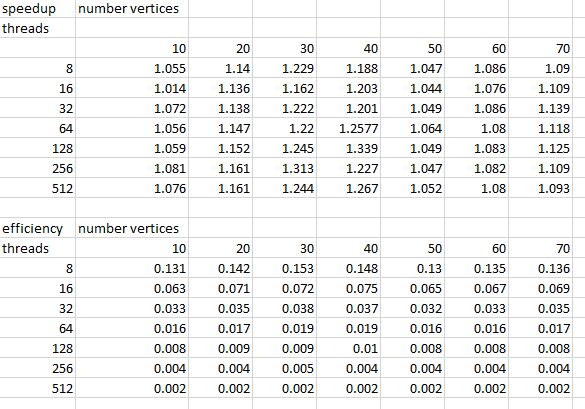
\includegraphics[width=4cm]{OpenMPTables.JPG}
    \caption{OpenMP speedup and efficiency graphs}
    \label{fig:my_label}
\end{figure}



\end{document}
